%% poster.tex
%% Vorlage fr A0-Poster
%% Harry Schmidt
%% 25.04.2003

%% translation instructions (there should be a better way):
%% latex ...
%% dvips -Ppdf -D9600 ...
%% psresize -w84cm -h118.8cm ... outfile.ps
%% edit postscript to position and size poster correctly
%%    bounding box in ps: 0 0 2380 3368
%%    after %%EndComments add:  gsave 0 -140 translate
%%    before showpage     add:  grestore
%% (adjust voffset and hoffset below to center text on page)
%% ps2pdf -sPAPERSIZE=a0 poster2a.ps


\documentclass{theo1poster}[2003/04/25]
\textwidth=11in                 % real width of latex text 
\textheight=11.3in                % height of latex text
\special{papersize=11.7in,12in}   % small width ensures portrait orientation
\addtolength{\voffset}{-.7in}
\addtolength{\textheight}{1.5cm}
\addtolength{\voffset}{52pt}  %% depends on actual length of poster
\addtolength{\hoffset}{8pt}   %% probably universal
%\usepackage[american,ngerman]{babel}
\usepackage[latin1]{inputenc}
\usepackage[T1]{fontenc}
%\usepackage{ae}
\usepackage{amsmath,amssymb,psfrag,pifont}
\usepackage{graphicx}

\input defs

%% Farben

\definecolor{lightblue}{rgb}{0.75,0.8,1}
\definecolor{graublau}{rgb}{0.85,0.85,0.9}
\definecolor{gruen}{rgb}{0.0,0.4,0.0}
\definecolor{alexblue}{rgb}{0.8,0.64,0.0}
\definecolor{strangeyellow}{rgb}{0.875,1.0,0.08}
\definecolor{verylightgray}{gray}{0.99}
\definecolor{meinrot}{rgb}{0.8,0.1,0.2}
\definecolor{lightocker}{rgb}{1,0.9,0.6}
\definecolor{orange}{rgb}{1,0.5,0}
\definecolor{darkorange}{rgb}{0.7,0.35,0}


\definecolor{sheetbg}{rgb}{0.75,0.8,1}
\definecolor{boxbg}{rgb}{1,1,0.95}
\definecolor{boxrahmen}{rgb}{0.11,0.15,0.4}


%% Stil-Befehle fr das Poster, kann fr jedes
%% einzelne Poster festgelegt werden

\posterbgcolor{sheetbg}    %% Hintergrundfarbe des Posters
%\posterbgcolor{lightocker}
%\posterbgcolor{lightblue}
%\posterbgcolor{graublau}


%\titlecolor{black}         %% Farbe des Titels
\headingcolor{black}       %% Farbe der �erschriften
%\headingcolor{meinrot}

%\headingfont{\sffamily}    %% Font der �erschriften
%\headingfontsize{\large}   %% Fontgr�e der �erschriften

\sheetframewidth{1mm}    %% Breite des Sheet-Rahmens
\sheetframesep{3pt}        %% Abstand des Textes vom Rahmen

\sheetframecolor{boxrahmen}    %% Farbe des Sheet-Rahmens
%\sheetframecolor{boxbg}
\sheetbgcolor{boxbg}       %% Farbe des Sheet-Hintergrunds
%\sheetbgcolor{verylightgray}

\colorsheets               %% Wird automatisch von \sheet..color  ausgefhrt
%\nocolorsheets             %% Default, solange \sheet..color nicht aufgerufen
%\roundsheets               %% Abgerundete Ecken ohne Farbe
\roundcolorsheets          %% Farbig und abgerundete Ecken

%\highlightcolor{lightocker} %% Farbe fr Hervorhebungen (Formeln)

%\renewcommand*\sectfont{\sffamily}
%\renewcommand*\sectfont{\bfseries\mathversion{bold}}

%\renewcommand*\bfdefault{b}


%% Sonstige Befehle

\renewcommand{\labelitemi}{\ding{228}}
\renewenvironment{itemize}% Liste mit bullet in gegebenem Abstand
                              % von linkem Rand der umschliessenden Umgebung
                              % M. Stollsteimer, 15.1.2001
 {\begin{list}{\labelitemi}%
       {%
%        \setlength{\topsep}{0pt}% Abstand vor Liste
        \setlength{\leftmargin}{0pt}% Raum vor bullet
        \setlength{\itemindent}{0pt}% Einrckung der ersten Zeile
        \settowidth{\labelwidth}{\labelitemi}%
        \addtolength{\labelsep}{\itemindent}
        \addtolength{\leftmargin}{\labelwidth}%
        \addtolength{\leftmargin}{\labelsep}%
        \addtolength{\leftmargin}{-\itemindent}%
       }%
 }
 {\end{list}}

\newenvironment{itemizenotopsep}{% Wie oben, nur mit \topsep=0pt
  \begin{list}{\labelitemi}%
    {%
      \setlength{\topsep}{0pt}% Abstand vor Liste
      \setlength{\leftmargin}{0pt}% Raum vor bullet
      \setlength{\itemindent}{0pt}% Einrckung der ersten Zeile
      \setlength{\itemsep}{0.5pt}% vertikaler Abstand von Items
      \setlength{\parsep}{1.5pt}%
      \settowidth{\labelwidth}{\labelitemi}%
      \addtolength{\labelsep}{\itemindent}
      \addtolength{\leftmargin}{\labelwidth}%
      \addtolength{\leftmargin}{\labelsep}%
      \addtolength{\leftmargin}{-\itemindent}}%
    }
  {\end{list}}


%% Daten fr den Titel

\title{State space geometry of a spatio-temporally\\ chaotic
Kuramoto-Sivashinsky flow}
\author{Predrag Cvitanovi\'c\ensuremath{^*}, Ruslan L. Davidchack\ensuremath{^\dagger} and Evangelos Siminos\ensuremath{^*}}
\newlength{\addresswidth}
 
\address{ \ensuremath{^*} Center for Nonlinear Science, Georgia Institute of Technology, 
          Atlanta, GA 30332-0430, USA\\
\ensuremath{^\dagger} Department of Mathematics, University of Leicester,
            University Road, Leicester LE1 7RH, UK
}


%\settowidth{\addresswidth}%
%       {\large Center for Nonlinear Science, Georgia Institute of Technology,}
%\address{\parbox{\addresswidth} {\centering%
%           Center for Nonlinear Science, Georgia Institute of Technology, 
%           Atlanta, GA 30332-0430, USA}%
%        }
%\logo{GT.eps}
%\setlength{\logowidth}{3cm}

%% Wem die Titelei nicht gef�lt:
%\renewcommand{\maketitle}{eigene Titelei}




\begin{document}


\begin{poster}{3}

\small

\begin{sheet}{Introduction}
In the dynamical systems approach, the
theory of turbulence for a given system, with given boundary conditions,
is given by (a) the geometry of the \statesp\ and (b) the associated natural measure,
\ie, the likelihood that asymptotic dynamics visits a given \statesp\ region.
We pursue this program in the context of \KS\ (KS) equation,
one of the simplest physically interesting spatially extended
nonlinear systems.

Dynamical \statesp\ representation of a PDE is $\infty$-dimensional,
but the KS flow is strongly contracting and its non-wondering set,
and, within it, the set of invariant solutions investigated here, is
embedded into a finite-dimensional inertial manifold\rf{FNSTks85} in
a non-trivial, nonlinear way. `Geometry' in the title of this paper
refers to our attempt to systematically triangulate this set in
terms of dynamically invariant solutions (\eqva, \po s, $\ldots$)
and their unstable manifolds, in a PDE representation 
independent way. The goal is to describe a given
`turbulent' flow quantitatively, not model it qualitatively by a
low-dimensional model.

In previous work, the \statesp\ geometry and the natural measure for
this system have been
studied\rf{Christiansen97,LanThesis,LanCvi07} in terms of unstable
periodic solutions restricted to the antisymmetric subspace of the
KS dynamics. The focus in this paper is on the role continuous symmetries play in
spatiotemporal dynamics.
The notion of exact periodicity in time is
replaced by the notion of relative spatiotemporal
periodicity, and \reqva\ and \rpo s here play the role the \eqva\
and \po s played in the earlier studies.  We undertake here
a study of the \KS\ dynamics for a specific system size $L = 22$, sufficiently large
to exhibit many of the features typical of `turbulent' dynamics
observed in large KS systems, but small enough to lend itself to a
detailed exploration of the  \eqva\ and \reqva,
their stable/unstable manifolds,
determination of a large number of
\rpo s, and a preliminary exploration of the relation between the
observed spatiotemporal `turbulent' patterns and the \rpo s.

\end{sheet}


\begin{sheet}{\KSe}

The \KS\ [henceforth KS] system\rf{ku,siv},
which arises in the description of
stability of flame fronts, reaction-diffusion systems and many other
physical settings, is one of the simplest nonlinear PDEs that
exhibit spatiotemporally chaotic behavior. In the formulation
adopted here, the time evolution of the `flame front slope'
$u=u(x,t)$ on a periodic domain $u(x,t) = u(x+L,t)$ is given by
\beq
  u_t = F(u) = -{\textstyle\frac{1}{2}}(u^2)_x-u_{xx}-u_{xxxx}
    \,,\qquad   x \in [-L/2,L/2]
    \,.
\ee{ks}
 In what follows
we shall state results of all calculations either in units of the
`dimensionless system size' $\tildeL$, or the system size $L = 2 \pi
\tildeL$. All numerical results presented in this paper
are for the system size $\tildeL=22/2\pi = 3.5014\ldots$.

\end{sheet}

\begin{sheet}{Symmetries of \KSe}

$G$, the group of actions $ g \in G $ on a
\statesp\ (reflections, translations, \etc) is a symmetry of the KS
flow \refeq{ks} if $g\,u_t = F(g\,u)$.
The KS equation is time translationally invariant, and space translationally invariant
on a periodic domain under
the 1-parameter group of
$O(2): \{\Shift_{\shift/L},\Refl \}$.
If $u(x,t)$ is a solution, then
\beq
	\Shift_{\shift/L}\, u(x,t) = u(x+\shift,t)
\ee{KSshift}
is an equivalent solution for any shift
$-L/2 < \shift \leq L/2$,
as is the
reflection (`parity' or `inversion')
\beq
    \Refl \, u(x) = -u(-x)
\,.
\ee{KSparity}

\end{sheet}

\begin{sheet}{\Eqva\ and \reqva}

\Eqva\  (or the steady solutions)
are the fixed profile time-invariant solutions,
\beq
 u(x,t) = u_\stagn(x)
\,.
\ee{eqva}
Due to the translational symmetry,
the KS system also allows for
\reqva\ (traveling waves, rotating waves),
characterized by a fixed profile $u_\stagn(x)$
moving with constant speed $c$, {\ie}
\beq
 u(x,t) =  u_\stagn(x-ct)
\,.
\ee{reqva}
Because of the reflection symmetry \refeq{KSparity},
the \reqva\ come in counter-traveling pairs
$u_\stagn(x-ct)$, $-u_\stagn(-x+ct)$.

\end{sheet}

\begin{sheet}{\Rpo s, symmetries and \po s} \label{sec:KSePO}

A relative periodic orbit satisfies
\beq
	g\, u(x,T_p)=u(x,0)\,,
\eeq
where $g\in G$, with $G$ a symmetry of the flow.
Thus, the KS equation can have relative periodic orbits corresponding
to 
\begin{enumerate}
 \item Invariance under $\Shift_{\shift/L}$
	\beq
		\Shift_{\shift_p/L}u(x,\period{p}) =
			u(x+\shift_p,\period{p}) = u(x,0) = u_p(x)\,.
		\label{KSrpos}
	\eeq
 \item Invariance under reflections 
	\beq
		\Refl u(x,\period{p}) =
			-u(-x,\period{p}) = u(x,0) = u_p(x)
			\,,
		\label{KSpos}
	\eeq
	Such an orbit is pre-periodic to a \po\ with period $2\period{p}$.
\end{enumerate}

\end{sheet}


\begin{sheet}{\Eqva\ and \reqva\ for $L=22$}
In addition to the trivial \eqv\ $u=0$ (denoted \EQV{0}),
we find three \eqva\ with dominant wavenumber $k$
(denoted \EQV{k}) for $k = 1, 2, 3$.  All {\eqva}  are symmetric with respect to the reflection
symmetry \refeq{KSparity}.
In addition, \EQV{2} and \EQV{3} are symmetric with respect
to translation \refeq{KSshift}, by $L/2$ and $L/3$, respectively.
\EQV{2} and \EQV{3} essentially lie, respectively, in
the 2$^\mathrm{nd}$ and 3$^\mathrm{rd}$ Fourier component complex plane,
with small $k=2j$, $k=3j$ harmonics deformations.

We find two pairs of \reqva\ \refeq{reqva} with velocities
$c =\pm 0.73699$ and $\pm 0.34954$
which we label \REQV{\pm}{1} and \REQV{\pm}{2},
for `traveling waves.' 

All \eqva\ and \reqva\ found here are unstable. Eventhough the \eqva\ lie in
the antisymmetric subspace, their unstable manifolds are not restricted to this subspace.

\centerline{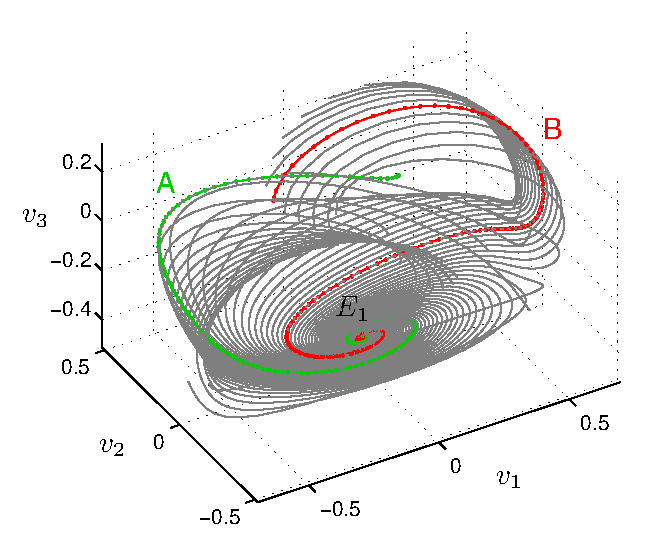
\includegraphics[width=.48\textwidth]{../../figs/ks22_E1_plane1_manifold_c.eps},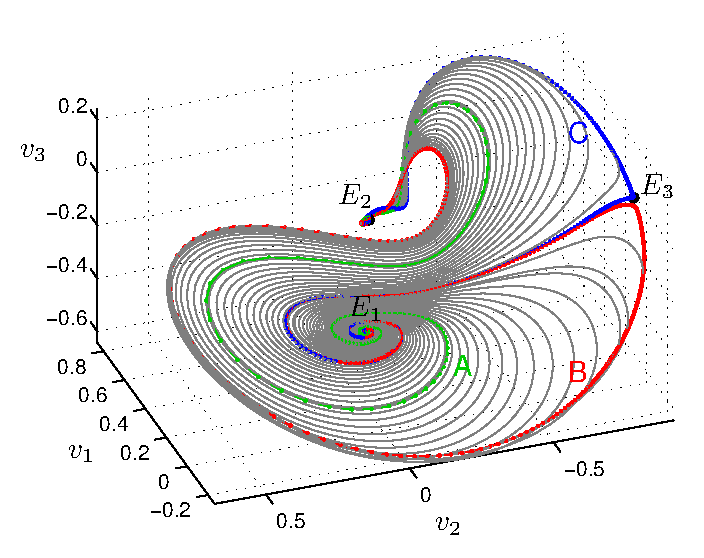
\includegraphics[width=0.48\textwidth]{../../figs/ks22_E1_plane2_manifold_c.eps}}
The left panel shows the unstable
manifold of \eqv\ \EQV{1} starting within the plane
corresponding to the first pair of unstable eigenvalues. 
% The
% coordinate axes $v_1$, $v_2$, and $v_3$ are constructed from vectors
% $\Re \,\jEigvec{1}$, $\Im \,\jEigvec{1}$,
% and $\Re \,\jEigvec{6}$
% by Gram-Schmidt orthogonalization. 
The right panel shows the unstable
manifold of \eqv\ \EQV{1} starting within the plane
corresponding to the second pair on unstable eigenvalues. 
% The
% coordinate axes $v_1$, $v_2$, and $v_3$ are constructed from vectors
% \Re\, $\jEigvec{3}$, \Im\, $\jEigvec{3}$, and \Re\, $\jEigvec{6}$
% by Gram-Schmidt orthogonalization.

\centerline{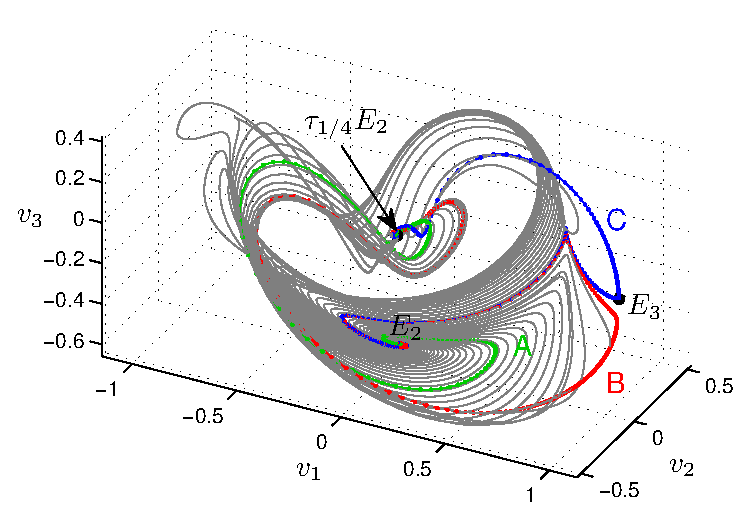
\includegraphics[width=.48\textwidth]{../../figs/ks22_E2_manifold_c.eps},\includegraphics[width=0.38\textwidth]{../../figs/ks22_E3_manifold.eps}}
The left panel shows the two-dimensional
unstable manifold of \eqv\ \EQV{2}. 
% The coordinate axes
% $v_1$, $v_2$, and $v_3$ are constructed from vectors
% \Re\, $\jEigvec{1}$, \Im\, $\jEigvec{1}$, and $\jEigvec{7}$
% by Gram-Schmidt orthogonalization.
 The right panel shows the two-dimensional
unstable manifold of \eqv\ \EQV{3}. 

The coordinate axes
$v_1$, $v_2$, and $v_3$ in all of the above figures are constructed by Gram-Schmidt orthogonalization from 
the stability eigenvectors corresponding to
the leading eigenvalues of the relevant equilibrium. 

The heteroclinic and homoclinic connections
between families of equilibria that can be seen in the figures are result of the symmetries of \KSe and are 
found to be structurally stable \refref{KNSks90}. 

\end{sheet}

\begin{sheet}{\Rpo s for $L=22$}
\begin{center}
\begin{tabular}{cccccc} (\textit{a}) & (\textit{c}) & (\textit{e}) &
                        (\textit{g}) & (\textit{i}) & (\textit{k})\\
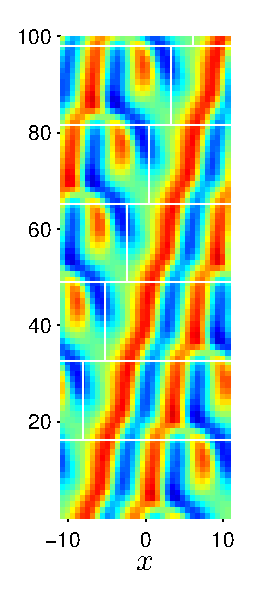
\includegraphics[width=0.15\textwidth]{../../figs/ks22rpo016.3-02.86.eps}\hspace{-4ex} &
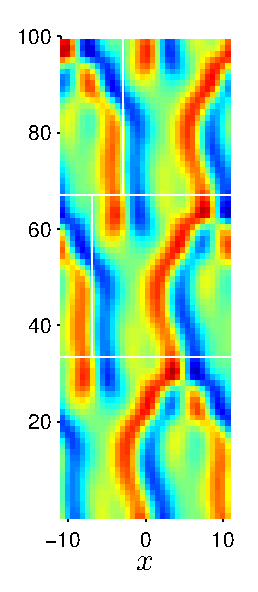
\includegraphics[width=0.15\textwidth]{../../figs/ks22rpo033.5-04.04.eps}\hspace{-4ex} &
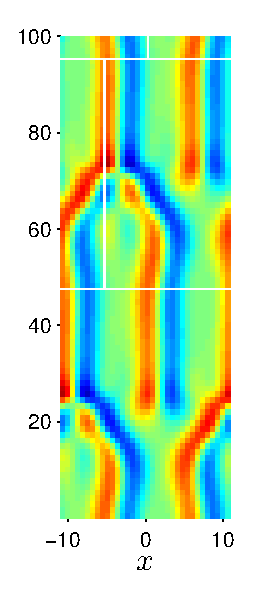
\includegraphics[width=0.15\textwidth]{../../figs/ks22rpo047.6-05.68.eps}\hspace{-4ex} &
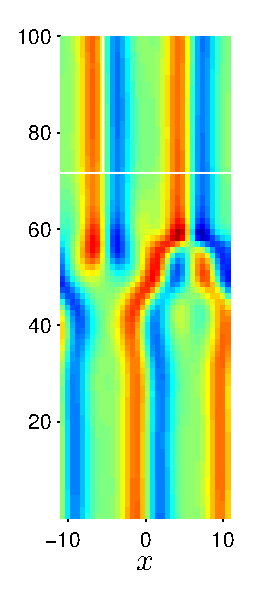
\includegraphics[width=0.15\textwidth]{../../figs/ks22rpo071.7-05.50.eps}\hspace{-4ex} &
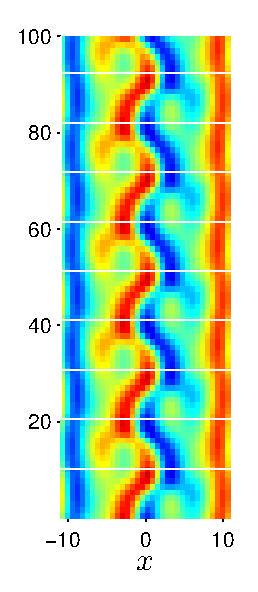
\includegraphics[width=0.15\textwidth]{../../figs/ks22rpo020.5-00.00.eps}\hspace{-4ex} &
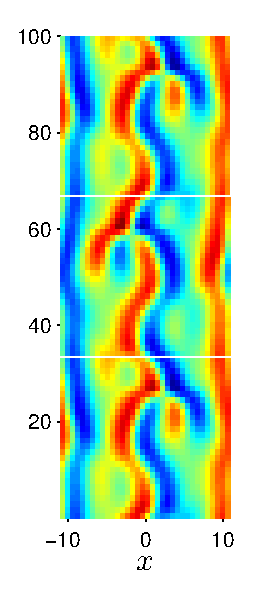
\includegraphics[width=0.15\textwidth]{../../figs/ks22rpo066.8-00.00.eps}\\
(\textit{b}) & (\textit{d}) & (\textit{f}) &
(\textit{h}) & (\textit{j}) & (\textit{l})\\
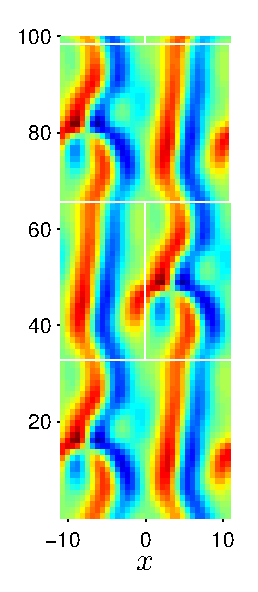
\includegraphics[width=0.15\textwidth]{../../figs/ks22rpo032.8-10.96.eps}\hspace{-4ex} &
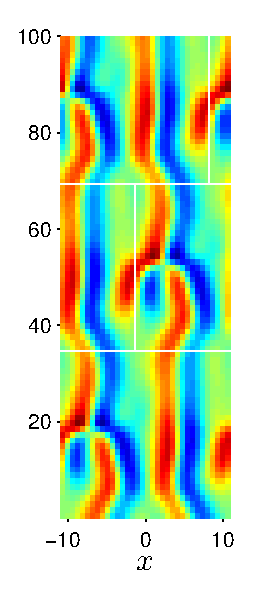
\includegraphics[width=0.15\textwidth]{../../figs/ks22rpo034.6-09.60.eps}\hspace{-4ex} &
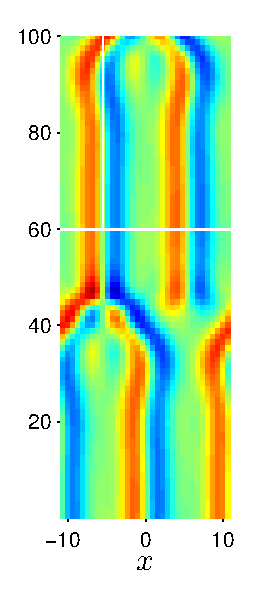
\includegraphics[width=0.15\textwidth]{../../figs/ks22rpo059.9-05.44.eps}\hspace{-4ex} &
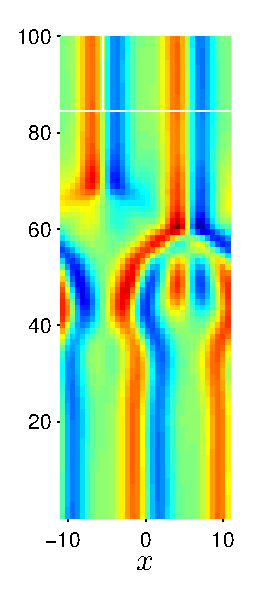
\includegraphics[width=0.15\textwidth]{../../figs/ks22rpo084.4-05.51.eps}\hspace{-4ex} &
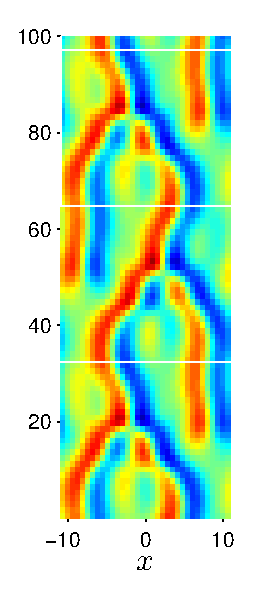
\includegraphics[width=0.15\textwidth]{../../figs/ks22rpo064.7-00.00.eps}\hspace{-4ex} &
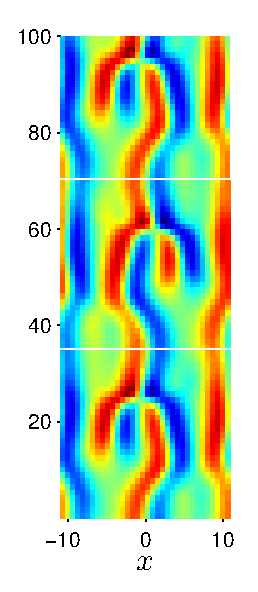
\includegraphics[width=0.15\textwidth]{../../figs/ks22rpo070.3-00.00.eps}
\end{tabular}
\end{center}
Selected relative periodic and
pre-periodic
orbits of \KSe\ with $L = 22$:
(a) $\period{p} = 16.3$, $\shift_p = 2.86$;
(b) $\period{p} = 32.8$, $\shift_p = 10.96$;
(c) $\period{p} = 33.5$, $\shift_p = 4.04$;
(d) $\period{p} = 34.6$, $\shift_p = 9.60$;
(e) $\period{p} = 47.6$, $\shift_p = 5.68$;
(f) $\period{p} = 59.9$, $\shift_p = 5.44$;
(g) $\period{p} = 71.7$, $\shift_p = 5.503$;
(h) $\period{p} = 84.4$, $\shift_p = 5.513$;
(i) $\period{p} = 10.3$;
(j) $\period{p} = 32.4$;
(k) $\period{p} = 33.4$;
(l) $\period{p} = 35.2$.
Horizontal and vertical white lines indicate periodicity and phase
shift of the orbits, respectively. We have limited our search to orbits with $\period{p} < 200$ and found
over 300 \rpo s with $\shift_p > 0$.
The search has not been exhaustive, and there are likely to be more
orbits with $\period{p} < 200$. However, the orbits we have found provide a representative sample of
typical periodic and \rpo s and approximate well the chaotic
attractor since they were located using seeds obtained from close
returns within the chaotic dynamics.

\end{sheet}


\begin{sheet}{Energy transfer rates for $L=22$}

\centerline{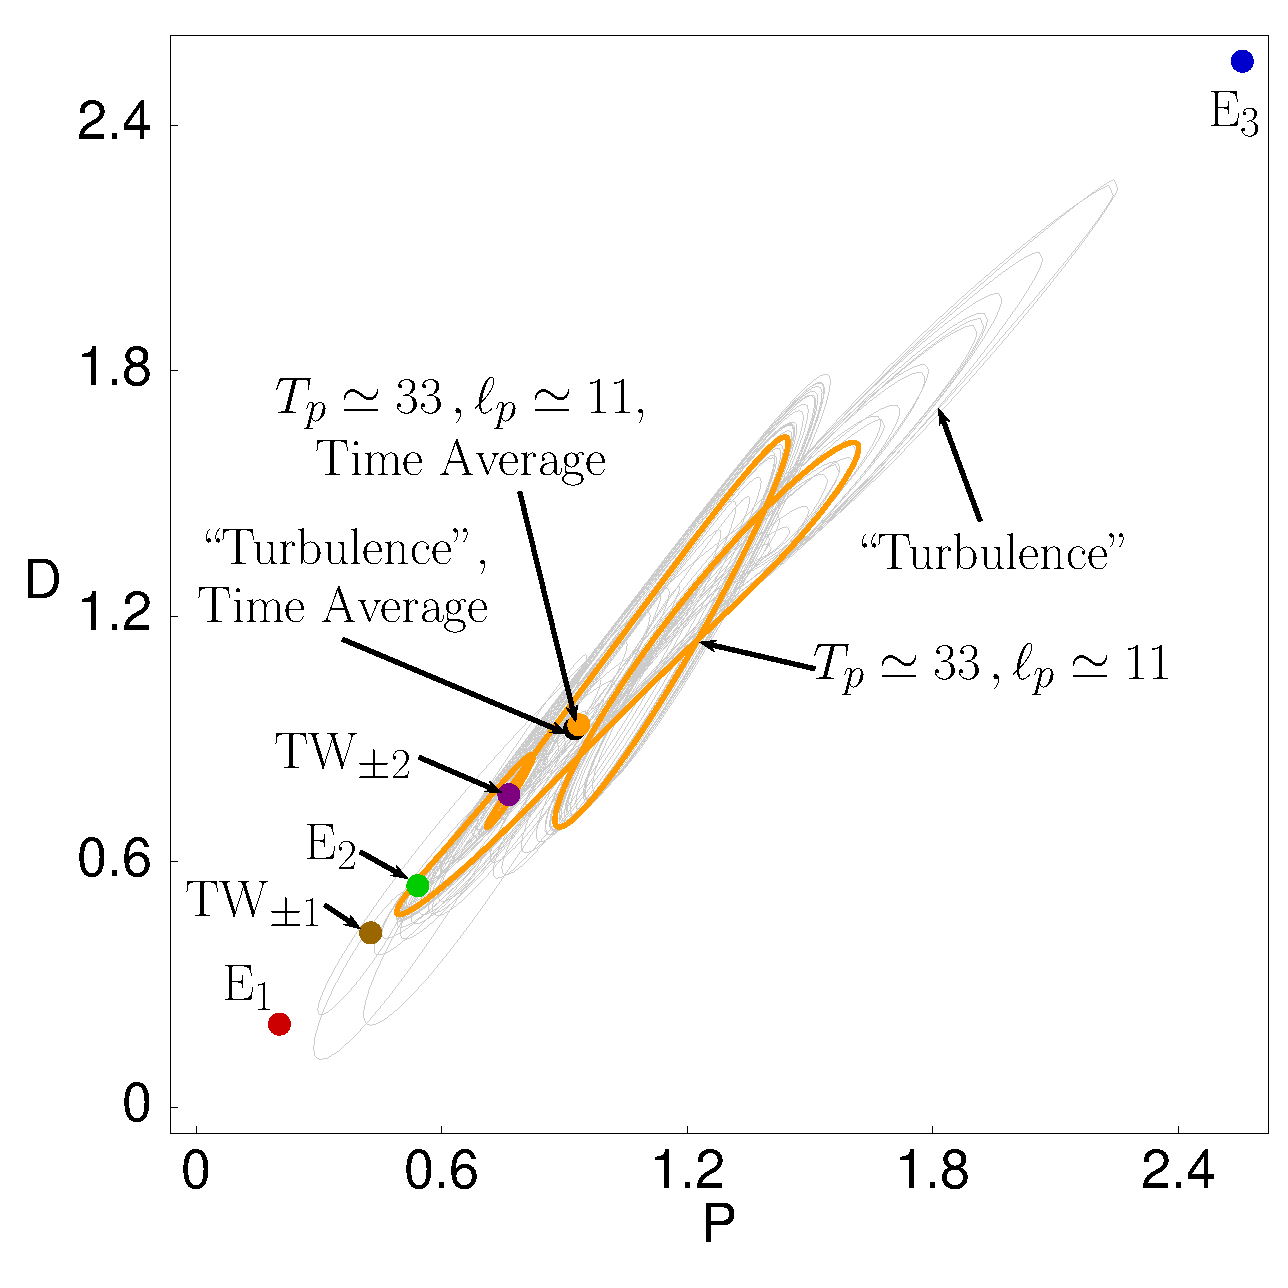
\includegraphics[width=.4\textwidth]{../../figs/energyBalance_pst.eps}}
Power input $P = \expct{u_{x}{}^2}$ {\em vs.}
dissipation rate  $D =  \expct{u_{xx}{}^2}$
for several  \eqva\ and \reqva,
a \rpo , and a typical `turbulent' long-time trajectory.
The \rpo\ $(\period{p},\shift_p) = (32.8,10.96)$ appears well embedded
within the turbulent flow. The mean power $\timeAver{P_p}$ 
is numerically quite close to the long-time
turbulent time average $\timeAver{P}$.
Yet, figures like this can be misleading. As always, here too one needs a hierarchy
of \po s of increasing length to obtain accurate
predictions\rf{DasBuch}.


\end{sheet}


\begin{sheet}{References}
\begin{thebibliography}{99}
 \bibitem{thisone}
	{\sc P.~Cvitanovi\'c, R.~L.~Davidchack and E.~Siminos},
	\emph{State space geometry of a spatio-temporally chaotic Kuramoto-Sivashinsky flow}, Submitted to
	SIADS J. Appl. Dyn. Systems (2007), arxiv.org/abs/0709.2944v1
\bibitem{FNSTks85}
{\sc C.~Foias, B.~Nicolaenko, G.~R. Sell, and R.~Temam}, C. R. Acad. Sci. I-Math, 301
  (1985), pp.~285--288.
\bibitem{LanThesis}
{\sc Y.~Lan}, PhD thesis, School of Physics, Georgia Institute of
  Technology, Atlanta, 2004.
\bibitem{LanCvi07}
{\sc Y.~Lan and P.~Cvitanovi\'{c}}, {\em Unstable recurrent patterns in
  {K}uramoto-{S}ivashinsky dynamics}.
{\sc Y.~Lan and P.~Cvitanovi\'{c}}, 
\newblock In preparation, 2007.
\bibitem{KNSks90}
{\sc I.~G. Kevrekidis, B.~Nicolaenko, and J.~C. Scovel},  SIAM J. Appl. Math., 50 (1990), pp.~760--790.
%\bibitem{ksgreene88}
%{\sc J.~M. Greene and J.~S. Kim},  Physica D, 33 (1988), pp.~99--120.
\bibitem{ku}
{\sc Y.~Kuramoto and T.~Tsuzuki},  Progr. Theor.
  Phys., 55 (1976), p.~365.
\bibitem{siv}
{\sc G.~I. Sivashinsky}, Acta Astr., 4
  (1977), p.~1177.
\bibitem{Christiansen97}
{\sc F.~Christiansen, P.~Cvitanovi\'{c}, and V.~Putkaradze}, Nonlinearity,
  10 (1997), p.~55.
\bibitem{DasBuch}
{\sc P.~Cvitanovi\'{c}, R.~Artuso, R.~Mainieri, G.~Tanner, and G.~Vattay}, {\em
  Chaos: Classical and Quantum}, Niels Bohr Institute, Copenhagen, 2005,
  ChaosBook.org.
\end{thebibliography}
\end{sheet}



\end{poster}


\end{document}
